\documentclass[pre,12pt]{revtex4-1}
\usepackage{float}
\usepackage{epsfig,graphics,amssymb,amsmath,subeqnarray,setspace,graphicx,amsthm,subfigure, mathrsfs,colortbl,color,bm,fancyhdr,wrapfig,tikz}

% Header on each page, with team number and page numbering
\pagestyle{fancy}
\lhead{Team \# 52821} 
\rhead{page \thepage \ of \pageref{LastPage}}
\cfoot{}
\renewcommand{\headrulewidth}{0.4pt}
\renewcommand{\footrulewidth}{0.0pt}

% Make life easier: define some shortcuts!
\def\b{\bm}
\def\e{\epsilon}
\def\ep{\varepsilon}
\def\u{\underline}
\def\c{\centerline}
\def\n{\noindent}
\def\h{\hangindent}


\newcommand{\tcb}{\textcolor{blue}}

% Double spacing is 2, 1.5 spacing is 1.5, ...
\def\baselinestretch{1.0}

% For tables:
\definecolor{Gray}{gray}{0.9}
\newcolumntype{C}{c<{\kern\tabcolsep}@{}}

\begin{document}

%\title{\textbf{Too Much Space Junk in Earth's Trunk: \\ \small A Data-driven Analysis of Space Debris Reduction}}
%\author{Team \# 52821}
%\date{\today}
%
%\maketitle

%%%%%%%%%%%%%%%%%%%%%%%%%%
\section{Introduction}\label{Introduction}

The issue of space debris has continued to grow in severity and impact since the publicized 2009 collision of the Russian satellite Kosmos-2251 and the USA satellite Iridium-33. These collisions can cost tens or hundreds of millions of dollars. Additionally, they threaten the safety of manned missions in the future of peaceful space exploration. There exists a great number of variables and parameters that factor into the time and spatial evolution of the space environment as well as numerous methods of debris reduction to consider. Thus, we aim to provide a model that applies to numerous situations and accounts for these processes. It can be adapted to include additional events to any degree of specificity. Our model simulates the population of space debris at various altitudes given the probability of these events. All parameters were selected based on research data to allow for the most accurate analysis of reduction methods, their benefits, and their costs.

%%%%%%%%%%%%%%%%%%%%%%%%%%
\section{Background}\label{Background}

Since the launch of Sputnik in 1957, the number of artificial objects orbiting the Earth has been steadily increasing. In 1978, Donald Kessler of NASA hypothesized that there exists a critical mass for space debris, above which the frequency of collisions and creation of new debris would cascade independently of further introduction of materials and Earth's orbital space would become too densely filled with debris for space travel to be feasible. This state is known as Kessler Syndrome.\cite{kesslerSyndrome} In the history of space travel, thousands of spacecraft have been sent into orbit. As of 2015, 696 are currently operational in Low Earth Orbit (LEO) \cite{satelliteDB}. The rest of the nonfunctional spacecraft have become large space debris. Space debris is constituted of more than just nonfunctional spacecrafts, as shown in Figure \ref{fig:classesOfSpaceObjects}. These objects are either released at the beginning of a mission (after launch), during the lifetime of a satellite, or the end of life of the satellite (breakups and/or malfunctions) \cite{orbitalDebris, studyOfOrbitalDebris}. All of this debris together contributes to the possibility of Earth being trapped in Kessler Syndrome. Whether the critical mass has been already been reached or not, it is clear that something must be done to reduce the amount of debris in space if extraterrestrial activites are to continue.

\begin{figure}[h!]
	\centering
    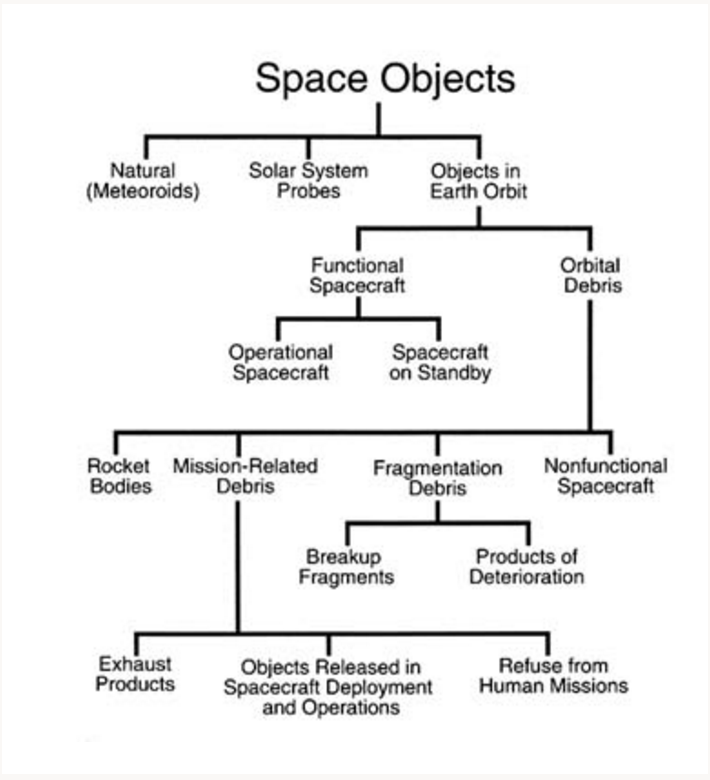
\includegraphics[width=0.35\linewidth]{figures/classesOfSpaceObjects.png}
    \caption{Classes of space objects orbiting the earth \cite{orbitalDebris}.}
    \label{fig:classesOfSpaceObjects}
\end{figure}

%%%%%%%%%%%%%%%%%%%%%%%%%%
\section{Assumptions}\label{Assumptions}

In the interest of combining simplicity and obtaining realistically relevant results, we made a number of assumptions. We believe that if we were to improve our model to relax these assumptions, our specific quantitative results would be affected, but not in a qualitative way. For example, further differentiation of the behavior of orbiting debris based on size would affect precise numbers of new debris created by collisions, but the trend of debris creation would remain quite similar. The following assumptions were utilized in our model to allow useful results to be obtained within the time allowed.

\begin{enumerate}
  \item Debris removal strategies should target LEO, where the current collision probability is orders of magnitude higher than upper altitudes\cite{orbitalDebris}. Our space debris model is restricted to activity in the LEO.
  \item LEO is the range of altitudes 200-1,600km.
  \item Operational satellites/spacecrafts stay at approximately the same altitude at which they were originally launched.
  \item The number of LEO launches per year is constant. This constant was obtained from the average number of LEO launches from the years $2000-2015$.
  \item The fraction of the total number of launches per year that go to the ISS (altitudes 370-460km) to the Sun Synchronous Orbit (SS-O) (600-800km) and to other altitudes (200-1600km) in LEO is constant. This constant fractions from the total number of launches were calculated using the number of launches from the years $2010-2015$ to these altitudes.
  \item The specific altitudes for yearly missions to the these destinations are uniformly distributed between their associated altitude range.
  \item The amount mission-related debris is constant across missions, and all of the debris released by the mission enters orbit at the altitude where the mission ends. For example, a mission to the ISS will create debris somewhere between 370-460km.
  \item The amount of debris obtained from Figure~\ref{fig:debris_density} at a certain altitude level is uniformly distributed throughout the level.
\end{enumerate}


While these assumptions may seem specific, we believe they do not limit the usefulness of our modeling results. Each assumption involves real data-derived constraints that we put into effect. We built a model based on these assumptions that gives a strong intuition and at least basic quantitative results for the query of space debris removal.

%%%%%%%%%%%%%%%%%%%%%%%%%

\section{The mathematical model}\label{Model}

\subsection{Overview}
We model the debris in LEO, the spacecraft that are launched there, and the interactions of these species as a chemical reaction network based on Continuous Time Markov Chains. The arrival of new spacecraft, the generation of new debris via collision as well as routine missions, and the removal of debris by reduction methods are stochastic point processes with rates and effects characterized by our research findings.

\subsection{Initial Conditions}
Before simulating debris reduction strategies in LEO, we had to determine the initial conditions of LEO debris and the number of operational satellites/spacecraft. To obtain an accurate measure of the current amount of debris in LEO we used the debris density distribution shown in Figure \ref{fig:debris_density} \cite{NasaLEODensity}. Since the debris density distribution originally was only available as a graphic, we used a web app called WebPlotDigitizer \cite{webPlotDigitizer} to extract usable data from it and integrate it into our model. The densely packed green stars in Figure \ref{fig:debris_density} are the interpolated discrete data points which we sampled to establish our model's initial conditions. Since we focused on untracked debris but sufficient data only existed for tracked debris, we used the tracked debris distribution from \cite{NasaLEODensity} coupled with a scale factor to match current estimates of total numbers of untracked debris in LEO.

In order to initialize the number of operational satellites/spacecrafts we downloaded the Union of Concerned Scientists (UCS) satallite database \cite{satelliteDB} and obtained the distribution of operational satellites in LEO shown in Figure \ref{fig:initDistOpSat}. Refer to Appendix~\ref{AppendixA} for detailed information about the satellite data.

\begin{figure}[h]
	\includegraphics[width=.8\linewidth]{"Figures/density_data"}
	\caption{\footnotesize LEO Debris Density}
	\label{fig:debris_density}
\end{figure}

\subsection{Initial Model - Orbital Decay}
In order to understand the impacts of debris removal from space, we first needed to understand the behavior of objects already in space. Objects in LEO are subject to orbital decay due to atmospheric drag \cite{orbitalDebris}. This means that objects in LEO are slowly falling towards Earth, making their orbital lifetime finite. While functional satellites are maintained at a desired altitude, other objects will eventually fall to Earth. Figure~\ref{fig:orbital_decay} shows curves of orbital lifetime for objects of various sizes introduced at various altitudes. The two dark solid lines represent the lifetimes of a 1cm object at the solar minimum and solar maximum. We use an average of these two lines for our object's orbital decay times. Our first model describes the orbital decay of the debris specified in the initial conditions.

\begin{wrapfigure}{l!}{0.4\textwidth}
	\vspace{-18pt}
	\includegraphics[width=\linewidth]{"Figures/orbital_decay"}
	\caption{Orbital decay}
	\label{fig:orbital_decay}
\end{wrapfigure}

Utilizing this data, we created a model that simulates the orbital decay of space debris over time if no new debris were introduced, including from collisions. The altitude range of interest (200km - 1600km) is segmented into levels which are treated as a set of interacting bodies, with objects from upper levels decaying into lower ones. Figure~\ref{fig:init_model} shows the result of this model with space discretized into 4 levels. We ran simulations with up to 20 levels for greatest fidelity of results, ultimately settling on using 6 levels to balance fidelity with computational speed and clarity. Without any sources of new debris, the debris in orbit in upper LEO slowly decays over time. The middle altitudes decay quickly, but reach an equilibrium sustained by the decay from upper altitude. The lower altitudes show similar effect, but the variations are quite pronounced since the decay rate is much faster. Discontinuities occur as the upper altitudes empty their debris. If the simulation were to be run for the length of the top orbital lifetime, the entire LEO region would empty. This of course ignores the effects of altitudes greater than $1,600$km. The orbital lifetimes increase exponentially with altitude; therefore, debris at these higher altitudes will orbit the Earth for thousands or even millions of years so we considered this effect negligible. For a quantitative measure of these lifetimes refer to Appendix \ref{AppendixC}.

\begin{figure}[h!]
	\includegraphics[width=.6\textwidth]{"Figures/Model1_4_10000"}
	\caption{Initial Model - Orbital decay}
	\label{fig:init_model}
\end{figure}


\subsection{Stochastics}
We improved upon our basic model by adding various possible events. These events include launch of new spacecraft, small fragments colliding with small fragments to create more fragments, and catastrophic collisions of fragments with spacecraft. We treated these events as point processes that trigger specific results from each event.
Our model may be represented with the following stochastic equation
\begin{equation}
	X(t) = X(0) + \sum_k Y_k \left(\int_0^t \lambda_k(X(s),s)ds\right) \zeta_k
\end{equation}

Where $X(t)$ is a vector of the quantity of space debris and space craft at time $t$, $Y_k$ are independent Poisson processes, $\lambda_k$ are intensity functions corresponding to each $\zeta_k$ reaction vector. The reaction vectors represent how a event in the model, e.g. a collision, affects the number of species. For example, a catastrophic collision vector would be
\begin{equation}
	\zeta = \begin{bmatrix} -1 \\ 2000 \end{bmatrix}
\end{equation}
since a catastrophic collision results in the lost of a spacecraft and the creation of approximately 2000 pieces of debris. For this vector, the corresponding $\lambda$ would signify the time frequency at which this particular catastrophic collisions take place. Each intensity function $\lambda_k$ can be a function of the variables and parameters of our choosing. Table~\ref{tab:lambdas} summarizes our choices for the dependence of each intensity function.

\begin{table}[h]
\centering
\begin{tabular}{r | c}
	Event Intensity & Depends on \\ \hline \hline
	Spacecraft Launch & Constant \\ \hline
	Catastrophic Collision & Number of Spacecraft and Debris \\ \hline
	Non-Catastrophic Collision & Number of Debris \\ \hline
\end{tabular}
\caption{$\lambda$ dependence}
\label{tab:lambdas}
\end{table}

\subsection{Second Model - Debris Collision}

The second model introduced collisions as a stochastic event. For the purposes of this paper, lethal debris will refer to debris in the size range 1cm - 10cm and spacecraft will refer to functional satellites. We chose to focus on this size range of debris because it is the range of debris that is untrackable but still capable of causing catastrophic collisions~\cite{lethal_debris}. There are two types of collisions that are of primary concern; fragment-fragment and spacecraft-fragment. We focus on the occurence of catastrophic collisions of fragments with spacecraft since these are of most value and result in the greatest number of new debris. 

An example of a catstrophic collision is the Iridium 33 and Cosmos 2251 collision from 2009. This was the first collision of two entirel spacecraft. Even with the massive increase in debris fragments due to the collision, the probability of another collision of this magnitude considering modern avoidance techniques is negligible \cite{IridiumProbs}. Therefore, we focus our modeling efforts on fragment-spacecraft collisions that may be impossible to avoid.


The amount of debris created from existing debris colliding with debris fragments or new launches is directly correlated to the debris density. A Lockheed Martin Space Operations team used NASA's elite LEGEND model to analyzed the probabilities of collisions from existing debris. The analysis was completing forecasting 100 years in the future. The results pertaining to shuttle-fragment and fragment-fragment collisions is summarized in Table \ref{table:CollisionAlt}. A resulting distribution over altitude (shown in Figure~\ref{fig:CollisionAlt}) corresponds to the existing LEO debris density distribution (shown in Figure~\ref{fig:debris_density}) \citep{CollisionProbs}. Although this data was used to model collisions for larger debris than the 1cm to 10cm range, the catastrophic parameter calculated using a similar model \cite{CollisionProbs2} is insignificant combined with the increase in spatial density for smaller debris.


\begin{table}[htb]
\centering
    \begin{tabular}{| c | c |} \hline
    \textbf{Collision Type} & \textbf{Number of Catastrophic Collisions} \\ \hline
    Shuttle-fragment & 12.4\\ \hline
    fragment-fragment & 0.9\\ \hline
    \end{tabular}
\caption{Collisions by Objects colliding in LEO orbit over 100 years}
\label{table:CollisionAlt}
\end{table}


\begin{figure}[h!]
	\includegraphics[width=.5\textwidth]{"Figures/CollisionAlt"}
	\caption{Impact Speed vs Collision Altitude for LEO collisions collected from LEGEND model for 30 Monte-Carlo runs predicting next 100 years\citep{CollisionProbs}.}
	\label{fig:CollisionAlt}
\end{figure}


To calculate the fragment increase accurately for each collision, many variables must be known or approximated. To simplify this step we assumed that a shuttle-fragment and fragment-fragment collision created constant 50,000 and 20 debris in the 1cm-10cm range respectively \cite{PhippsSpaceLaserNudge}. These values were chosen due to their corresponding impact parameters, velocities, and to mirror similar results of collisions and explosions \citep{CollisionProbs2} \citep{Explosion1}. The results compared to the initial model will be analyzed within the third model.

\subsection{Third Model - Spacecraft Launches}

Building upon Model 2 we introduced yearly LEO spacecraft launches as stochastic events. These events will introduce a satellite to one of the levels in LEO and a constant amount of debris to that same level. There were three main components that we had to characterize in order to incorporate spacecraft launches into our model.\\

\textbf{Target Level: }In order to determine the altitude level at which a launch would arrive, we surveyed the Space Launch Report yearly log files \cite{spaceLaunchReport}. First, we studied the log files from 2000-2015 and calculated the average launches to LEO. Then we examined how these launches were categorized in the log files. These were: LEO/ISS, LEO/SS-O, and LEO (which we refer to as LEO/Other). Using data from 2010-2015 we calculated the average number of launches to each of these categories (ISS, SS-O and Other). The third step was to calculate the ratio of each of the three possible categories to the total number of launches in a year. The calculated ratios can be found in Table \ref{launchRatios}.  Finally, using the determined target place we could find the altitude by generating a uniform random variable between the altitude ranges in Table \ref{altitudeRanges}.  \\
\begin{table}[h]
\centering
    \begin{tabular}{| c | c | c | c |}     
    \hline
    \textbf{Avg. LEO Launches Per Year} & \textbf{Ratio of LEO/ISS} & \textbf{Ratio of LEO/S}  & \textbf{Ratio of LEO/Other}\\ \hline
    36.4375 & 0.2850 & 0.3842 & 0.3308\\ \hline
	\end{tabular}
\caption{Calculated ratios from data in Appendix \ref{AppendixB}.}
\label{launchRatios}
\end{table}

\begin{table}[h]
\centering
    \begin{tabular}{| c | c | c |}     
    \hline
    \textbf{LEO/ISS (km)} & \textbf{LEO/SS-O (km)} & \textbf{LEO/Other (km)} \\ \hline
    $370-460$ & $600-800$ & $200-1600$ \\ \hline
	\end{tabular}
\caption{Altitude ranges used to determine which level a given launch ends up in. ISS range was obtained from \cite{esaISS} and SS-O range was determined by noting that the largest number of operational satellites orbit at those altitudes.}
\label{altitudeRanges}
\end{table}

\textbf{Launch Rate Per Level: } In order to determine the launch rate and incorporate it as a stochastic event, we used the target level results. Every 365 days we would generate a distribution of launches to each altitude level using the data and results from the target level section. Using this distribution we could calculate the stochastic launch rates per level. These remain constant for the following simulated year. This accounts for both the variation and consistency seen in the data from the past 15 years. \\

\textbf{Amount of released debris: }Our model takes the amount of debris released per launch as a constant. We set this constant to $70$ because according to \cite{orbitalDebris} a detailed study of a Russian launch mission determined that $76$ different objects were put into orbit. We treated this as an upper bound and settled on 70 as a reasonable average amount that is close to a worst case scenario in order to challenge our model. \\

\subsection{Fourth Model - Debris Reduction}

The final iteration of our model included a debris reduction variable. The variable was added to the model as a stochastic event signifying the average rate of debris removal per time unit of the process. This approach provides an ease for testing single processes or any number of combinations, while also allowing for careful numerical analysis of the reduction process' effect for different altitudes.

With initial research, we realized that there were many substantially researched debris reduction processes. A non-exhaustive breakdown of debris capture and reduction methods are shown in Figure \ref{fig:ReductionMethods}.

\begin{figure}[h!]
	\includegraphics[width=1\textwidth]{"Figures/ReductionMethods"}
	\caption{A breakdown of debris capture and reduction methods \citep{ReductionMethods}.}
	\label{fig:ReductionMethods}
\end{figure}


We chose to focus on a small number of these processes due to the vast array of distinct reduction methods. After initial reduction research we found that any process utilizing direct capture of debris requires a spacecraft to match debris velocity. This requires a great amount of energy to reduce a small number of lethal debris. While the cost models for these other processes are not fully developed for LEO debris, many can be modeled using Bannal's estimate of 27 million dollars per object \citep{PhippsRemovingDebris}. Applying this to lethal debris sizes gives similar cost estimates. Since laser based removal systems don't have this requirement and also have an abundance of recent research, we decided to focus our efforts on those reduction processes alone. With the model, other reduction processes can easily be used and compared.

Investigation of laser techniques revealed many internal dependencies for the cost and reduction functions. An initial cost and reduction analysis would be to compare energy usage of the laser, energy needed to remove a single debris target, and the time taken to complete this task. While this would work provide a rough estimate, much more sophisticated cost and reduction analysis has already been computed at Photonic Associates LLC, taking into account numerous factors, such as laser mirror sizes, laser energy and pulse ranges, target size and mass, target altitude, laser down time, and laser tracking time among others. The results from multiple optimized models are compiled below in Table \ref{table:Lasers}.
 
\begin{table}[htb]
\centering
	\begin{tabular}{||c|c|c|c|c|c||} \hline
	\textbf{Model} & \textbf{\shortstack{Removal Rate \\ (debris/yr)}} & \textbf{\shortstack{Cost Rate \\  (M/yr)}} & \textbf{\shortstack{Target Range \\ $\pm$ 200 (km)}} & \textbf{\shortstack{Target Mass \\ (kg)}} & \textbf{\shortstack{Ground vs \\ Spaced Based \\ (G/S)}} \\ \hline
	A \cite{ORION} & 15,000 & 93 - 108 & 800 & $< 1cm$ & G \\ \hline
	B \cite{ORION} & 38,333 & 140 - 176 & 1500 & $< 1cm$ & G \\ \hline
	C \cite{PhippsSpaceLaserNow} & 20,000 & 240 & 1000 & 0.75 & G \\ \hline
	D \cite{PhippsSpaceLaserNow} & 202 & 953 & 800 & 750 & G \\ \hline
	E \cite{PhippsSpaceLaserNow} & 75 & 397 & 800 & 1400 & G \\ \hline
 	F \cite{PhippsSpaceLaserNow} & 260,000 & 80 & 760 & 0.083 & S \\ \hline
	G \cite{PhippsSpaceLaserNow} & 500 & 140 & 600 & 1000 & S \\ \hline
	\end{tabular}
\caption{Compares different laser models}
\label{table:Lasers}
\end{table}

%%%%%%%%%%%%%%%%%%%%%%%%%

\section{Numerical methods}\label{Numerics}

Two different numerical methods were merged in order to simulate our space debris model. Orbital decay is a deterministic process and was modeled in that fashion, while the occurence of the other events in our model was stochastic based. These two processes needed to work in harmony in order for our model to function.

We desired to ensure that without any introduction of debris, our simulated space would be empty of debris in the time frame of the longest orbital lifetime. Thus, given an initial distribution of space debris across altitudes~\cite{orbitalDebris} we created a simluated history of those objects spread over the length of the orbital lifetime, in a uniform random distribution. For example, at an altitude with an orbital lifetime of 10 days with 1000 initial pieces of debris will lose an average of 100 pieces of debris to decay per day such that this altitude will be empty on day 10. However, any new objects added to that altitude will be accounted for and begin to decay at the same rate.

The stochastic aspects of our simulations utilized a next reaction algorithm, a standard and efficient method of simulating Continuous Time Markov Chains. For each time step, the intensity functions are calculated and used to scale an exponential random variable. This scaling is tracked for each iteration so that the intensities accumulate for each reaction. The reaction with the highest cumulative intensity is chosen as the next reaction, and the length of the time step is chosen to be the exponential random variable (RV) scaled by that chosen intensity function. That cumulative intensity is reset by that exponential RV and the process continues. Using exponential random variables in this way ensures that the Markov memoryless property is satisfied, while the desired rates and averages of each event is controlled and behaves to expectation. The exact mathematics is shown below.

\begin{enumerate}
	\item $P$ and $T$ are initialized, $P$ as a vector of exponential random variables and $T$ as a vector of zeros
	\item $\lambda$s calculated based on Table \ref{tab:lambdas}
	\item $\Delta T$ is set to $\frac{P - T}{\lambda}$, an element-wise division
	\item $\inf(\Delta T)$ is chosen to be the time step $\Delta t$, while the corresponding reaction is the next reaction, $k$
	\item The reaction vector $\zeta_k$ is returned
	\item T is updated to $T + \Delta t \lambda$ 
	\item $P_k = P_k + Y_i$, a new exponential RV chosen for each iteration
	\item Steps 2-7 are repeated for the duration of the simulation
\end{enumerate}
We used units of days for our intensities. This fine scaling allowed high fidelity for these processes that were run for tens of thousands of days.

%%%%%%%%%%%%%%%%%%%%%%%%%%
\section{Results and analysis}\label{Results}

To see the effects of our chosen debris removal strategy over time, we compared two key statistics from running simulations for a 100 year span. Without any debris reduction, current estimates are that there will be 12.4 catastrophic collisions during that time~\cite{CollisionProbs}. Our model was run and calibrated to match that result on average. A sample simulation result is shown in Figure~\ref{fig:traj_no_reduce}. This simulation was run 15 times to ensure our model parameters matched those predicted. We then iterated over a range of debris removal amounts and recorded the number of catastrophic collisions as well as the net change in debris amounts in LEO. Figures~\ref{fig:reducecol} and~\ref{fig:diffdebris} show the results of these simulations. 5 repetitions of each removal amount was averaged. In addition, a set of simulations was run with the debris removal set to its maximum amount but only for the first 5 years. Figure~\ref{fig:traj_5yr_reduce} shows a sample result of this simulation, and Table~\ref{tab:results} summarizes the results of all simulations.

\begin{figure}
	\hspace*{-40pt}
	\includegraphics[width=1.2\linewidth]{"Figures/traj_no_reduce"}
	\caption{A single trajectory of a simulation with no debris removal. Debris is on the left while the corresponding spacecraft in that level is on the right. Occurences of catastrophic collisions are denoted by a red asterisk.}
	\label{fig:traj_no_reduce}
\end{figure}

\begin{figure}
	\hspace*{-40pt}
	\includegraphics[width=1.2\linewidth]{"Figures/traj_5yr_reduce"}
	\caption{A single trajectory of a simulation with debris removal at the theoretical maximum amount of 712/day for 5 years, then none for 95 years.}
	\label{fig:traj_5yr_reduce}
\end{figure}

\begin{table}[h]
\centering
\begin{tabular}{| r | c| c| c|} \hline
	Avg Daily Removal Amount & Avg Debris Change & Avg Catastrophic Collisions & Standard Deviation \\ \hline
	0 & 60247 & 11.2 & 4.89 \\ \hline
	8 & 7495 & 8 & 5.24 \\ \hline
	16 & -19925 & 8.4 & 4.16 \\ \hline
	32 & -107733 & 2.6 & 2.07 \\ \hline
	64 & -104532 & 0.8 & 1.10 \\ \hline
	128 & -107632 & 0.8 & 0.84 \\ \hline
	256 & -105705 & 1.0 & 1.22 \\ \hline
	712 & -100216 & 1.0 & 1.00 \\ \hline
	712/5yr & -61117 & 2.8 & 4.6 \\ \hline
\end{tabular}
\caption{Simulation Results}
\label{tab:results}
\end{table}

\begin{figure}[h!]
	\includegraphics[width=.75\textwidth]{"Figures/results_collisions"}
	\caption{The predicted number of catastrophic collisions drops quickly with debris removal}
	\label{fig:reducecol}
\end{figure}
\begin{figure}[h!]
	\includegraphics[width=.75\textwidth]{"Figures/results_difference"}
	\caption{With only a small amount of daily debris removal, significant changes can be made to the amounts in LEO}
	\label{fig:diffdebris}
\end{figure}


%%%%%%%%%%%%%%%%%%%%%%%%%%%%%%
\section{Discussion}\label{Discussion}

Our results indicate that a low threshold of debris removal on a daily basis can have substantial effects on future catastrophic collisions and the environment of debris as a whole. While some sources claim to be able to affordably remove LEO space debris by 260,000 objects per year, we found that removing as little as 12,000 per year can reduce future catastrophic collisions by 8.6. Additionally, we were able to predict similar benefits between small amounts of debris reduced for 100 years and a large amount of debris removal for 5 years. This is vitally important information for any private enterprise interested in space debris removal. The catastrophic collisions involve spacecraft that are expensive to build, launch, and maintain. Not needing to replace these destroyed spacecraft provides savings of hundreds of millions of dollars. This provides a massive incentive for a private company to take on the challenge of space debris removal. 

While our model can be furthered refined to ensure its results are most accurate and precise, its qualitative conclusion is unlikely to change. Space debris is certainly a problem that is solvable in our lifetimes.

\subsection{Strengths of the model}

\begin{itemize}
	\item Our model is data-driven and agrees with multiple long term studies given zero reduction factor
	\item The model is able to be applied effortlessly to any number of additional events
	\item The model is able to target and model specific altitude ranges providing increased forecasting precision
	\item While the results are limited by the precision of the cost models, as research progress in those areas, the model will be able to handle any number or combination of reduction scenarios
\end{itemize}
 

\subsection{Weaknesses of the model}

\begin{itemize}
	\item The model's precision is dependent on the relationship between large and small debris in LEO, which was approximated from sample data
	\item The model considers few of the many reduction processes
	\item While the assumptions are fair, the model does not account for debris outside of LEO or for variation in debris size and mass 
\end{itemize}

\subsection{Future directions}


There are three components, in our opinion, that would strengthen our model.

\begin{enumerate}
	\item \textbf{Support for variable Debris Size: }Space Debris can be categorized in small ($<1cm$), medium or lethal ($1-10cm$), and large ($>10cm$). The number of each type of debris fragments greatly varies between categories and pose different kinds of threats to operational spacecraft. Small particles can produce more small particles when colliding with spacecraft or large-sized debris. Medium-sized can produce breakups or even explosions in operational spacecraft. Finally, large debris fragments have the highest probability of destroying operational spacecraft upon collisions. Therefore, this would be a very important step to a precise characterization of the time evolution of space debris.
	\item \textbf{Validation of Data: }All of the data used during initialization and throughout the time evolution was obtained from reputable sources. Being able to validate the data, however, would be highly beneficial. Numbers such as the initial debris concentration, spacecraft launch altitudes, or the amount of mission-related debris could be further refined to make our model as robust as possible.
	\item \textbf{Evaluation of more Debris Removal Strategies: } Our model determined that if we are able to remove a certain amount of debris per day we can prevent LEO debris to reach the critical mass described in Kessler's Syndrome. Therefore, the next step is to further quantitatively evaluate debris removal technologies and determine the most effective and economically feasible strategy.  
\end{enumerate}


\clearpage

\bibliographystyle{unsrt}
\bibliography{ThePaper}

\clearpage
\appendix

\section{Operational Satellite Data}\label{AppendixA}

Our model initialized the number of operational satellited in LEO using data obtained from the Union of Concerned Scientists (UCS) Satellite Database \cite{satelliteDB}. According to \cite{satelliteDB} there are 696 functional satellites in orbit as of 8/31/15, whose altitudes are distributed as depicted in Figure \ref{fig:initDistOpSat}. Our level-based debris model initializes places these satellites in different levels depending on the altitude.

\begin{figure}[h!]
	\includegraphics[width=.8\textwidth]{"Figures/initDistributionOfOperationalSatellites"}
	\caption{Initial distribution of operational satellites in LEO as specified by the UCS Satellite Database.}
	\label{fig:initDistOpSat}
\end{figure}

\clearpage
\section{Launch Data}\label{AppendixB}

The amount of mission-related debris that is produced every year is proportional to the number of yearly launches. In order to calculate a reasonable measure for mission-related debris we had to first gather yearly LEO launch data. Furthermore, we had to estimate where in the LEO this debris would end up to determine in which level of our model it would end up. To this end we classified LEO launches as either: ISS (International Space Station), SS-O (Sun-Synchronous Orbit) or Other. Other launches are the ones that were not cataloged as either ISS or SS-O. The following tables contain the data gathered from \cite{spaceLaunchReport}, that was used to calculate an average number of launches and the percentage of the launches that go to either the ISS, SS-O or some other LEO altitude.
\
\begin{table}[htb]
    \begin{tabular}{| c | c | c |} \hline
    \textbf{Year} & \textbf{LEO Launches} & \textbf{Total Launches} \\ \hline
    2000 & 33 & 85 \\ \hline
    2001 & 27 & 59 \\ \hline
    2002 & 31 & 65 \\ \hline
    2003 & 25 & 63 \\ \hline
    2004 & 26 & 54 \\ \hline
    2005 & 29 & 55 \\ \hline
    2006 & 33 & 66 \\ \hline
    2007 & 36 & 68 \\ \hline
    2008 & 36 & 68 \\ \hline 
    2009 & 45 & 78 \\ \hline
    2010 & 37 & 74 \\ \hline
    2011 & 43 & 84 \\ \hline
    2012 & 40 & 78 \\ \hline
    2013 & 48 & 81 \\ \hline
    2014 & 50 & 92 \\ \hline
    2015 & 44 & 86 \\ \hline
    \end{tabular}
\caption{Launch data obtained from the Space Launch Report log files \cite{spaceLaunchReport}.}
\end{table}

\begin{table}[htb]
\centering
    \begin{tabular}{| c | c | c | c |} \hline
    \textbf{Year} & \textbf{LEO ISS Launch} & \textbf{LEO SS-O Launch}  & \textbf{LEO Other Launch} \\ \hline
    2010 & 12 & 12 & 14\\ \hline
    2011 & 13 & 17 & 13\\ \hline
    2012 & 12 & 14 & 14\\ \hline
    2013 & 12 & 16 & 20\\ \hline
    2014 & 13 & 23 & 14\\ \hline
    2015 & 12 & 18 & 11\\ \hline
    \end{tabular}
\caption{LEO Launch data obtained from the Space Launch Report log files. ISS: International Space Station; SS-O: Sun Synchronous Orbit; Other: Not specified \cite{spaceLaunchReport}.}
\end{table}

\clearpage
\section{Altitude vs. Decay Times Extrapolation}\label{AppendixC}
The data in Figure \ref{fig:orbital_decay} only shows us the decay times up to $~1,000$km. The length of our final simulations were around a $100-200$ years ($365,000-730,000$ days). This means that all of the initial debris in the higher levels will have completely decayed. Therefore we decided to extrapolate the data so it would contain altitudes up to $2,000$km as shown in \ref{fig:altDecayTimesExtrapolated} so that not even in the longest simulations we have the debris from the higher levels reach the first level.

\begin{figure}[h]
\centerline{%
\includegraphics[height=6cm, width=0.5\textwidth]{"Figures/extrapolatedAltDecayTimes"}%
\includegraphics[height=6cm, width=0.5\textwidth]{"Figures/altDecayTimesWithAddedData"}%
}%
\caption{Left: Altitude vs Decay Times data with trendline. Right: Altitude vs Decay Times sample from both original data and extrapolated data of Left. Samples from from 175-1,000 km come from the original data and the sample from 1,000-2,000 km come from the trendline.}
\label{fig:altDecayTimesExtrapolated}
\end{figure}


\clearpage

\end{document}

